\section{Modellierung eines Embedded Systems}

\subsection{V-Modell für Software-Entwicklungszyklus}

\begin{center}
    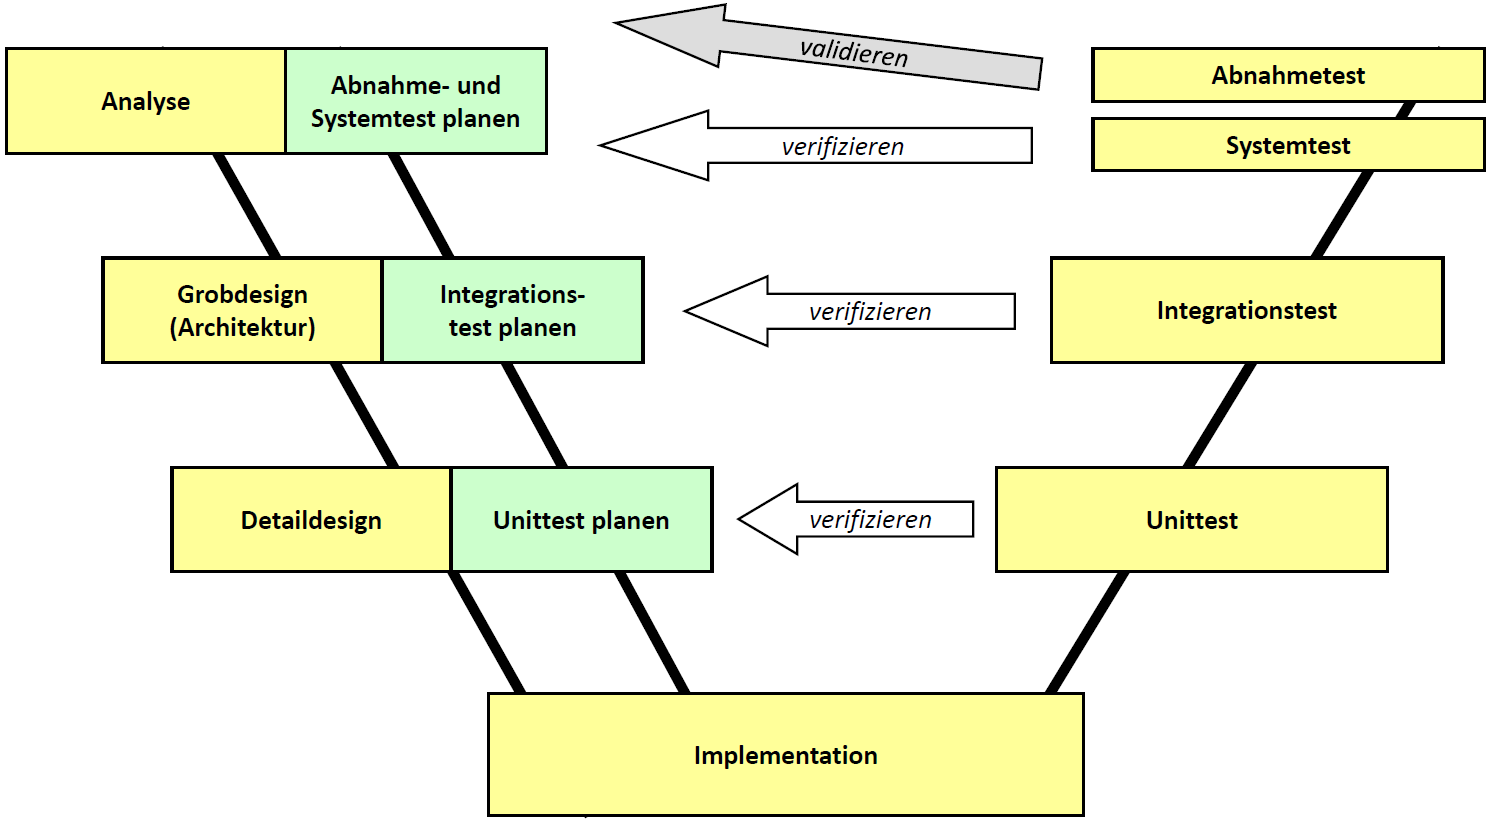
\includegraphics[width=0.7\columnwidth]{images/V_modell.png}
\end{center}

\textrightarrow\ Nur Anforderungen (requirements) definieren, welche man auch testen kann!


\subsection{Model Driven Development (MDD)}

\begin{outline}
    \1 Bei \textbf{modellbasierter Entwicklung} kommen in \textbf{allen Entwicklungsphasen} durchgängig Modelle zum zur Anwendung
    \1 MDD geht davon aus, dass aus formalen Modellen lauffähige Software erzeugt wird \\
        \textrightarrow\ Codegeneratoren
    \1 Modelle werden traditionell als Werkzeug der Dokumentation angesehen
        \2 Unter Umständen wird zweimal dasslbe beschrieben (Code und Diagramm) \\
            \textbf{\textrightarrow\ unbedingt zu vermeiden!}
\end{outline}


\subsection{Vorgehen bei der Modellierung}

\begin{minipage}[c]{0.6\columnwidth}
    \begingroup
    \renewcommand{\outlinei}{enumerate}
    \renewcommand{\outlineii}{itemize}

    \begin{outline}
        \1  \cgn{Systemgrenze definieren}
            \2 Kontextdiagramm: Use-Case-Diagramm
            \2 Kontextdiagramm: Sequenzdiagramm
        \1 \cgn{Systemprozess finden}
            \2 Kontextdiagramm: Use-Case-Diagramm
            \2 Kontextdiagramm: Sequenzdiagramm
        \1 \cgn{Verteilungen festlegen}
            \2 Verteilungsdiagramm (deployment diagram)
        \1 \cbl{Systemprozesse detaillieren}
            \2 Umgangssprachlicher Text
            \2 Sequenzdiagramm
            \2 Aktivitätsdigramm
            \2 Statecharts
            \2 Code (C, C++, ...)
    \end{outline}
    \endgroup
\end{minipage}
\hfill
\begin{minipage}[c]{0.38\columnwidth}
    \raggedright
    \cgn{Stukturmodellierung (Statische Aspekte)}
    
    \vspace{0.2cm}

    \cbl{Modellierung der dynamischen Aspekte}
\end{minipage}


\subsection{Systemgrenze definieren \& Systemprozesse finden}

\subsubsection{Systemgrenze definieren}

\textbf{Die Festlegung der Systemgrenze ist das Wichtigste und Allererste bei sämtlichen Systemen!}

Man sollte sich die folgenden Fragen stellen und diese beantworten:

\vspace{0.1cm}

\begin{outline}
    \1 Was macht das System, d.h. was liegt innerhalb der Systemgrenze?
        \2 Was macht das System  \textbf{nicht}?
    \1 Mit welchen Teilen ausserhalb des Systems kommuniziert das System?
    \1 Welches sind die Schnittstellen zu den Nachbarsystemen (Umsystemen, periheral system)?
\end{outline}


\subsubsection{Systemprozesse finden (use-cases)}

Da man sich noch immer in der \textbf{Analyse} befindet, sollen nur die \textbf{Anforderungen} definiert werden. Die Umsetzung ist Teil
des Designs! \\
Um die Use-Cases zu identifizieren, sollte folgendes beachtet werden:

\vspace{0.1cm}

\begin{outline}
    \1 Aussenbetrachtung des Systems (\textbf{oberflächlich!})
        \2 Nicht komplizierter als nötig
    \1 System als Blackbox betrachten 
        \2 \textbf{Was} soll System können; (nicht: wie soll das System etwas machen)
    \1 RTE-Systeme bestehen häufig aus nur einem einzigen Systemprozess 
        \2 speziell wenn System 'nur' ein Regler ist
\end{outline}


\subsubsection{Kontextdiagramm: Use-Case Diagramm}

\begin{minipage}[t]{0.4\columnwidth}
    \myul{\textbf{Tempomat: zu detailliert}}

    \vspace{0.1cm}

    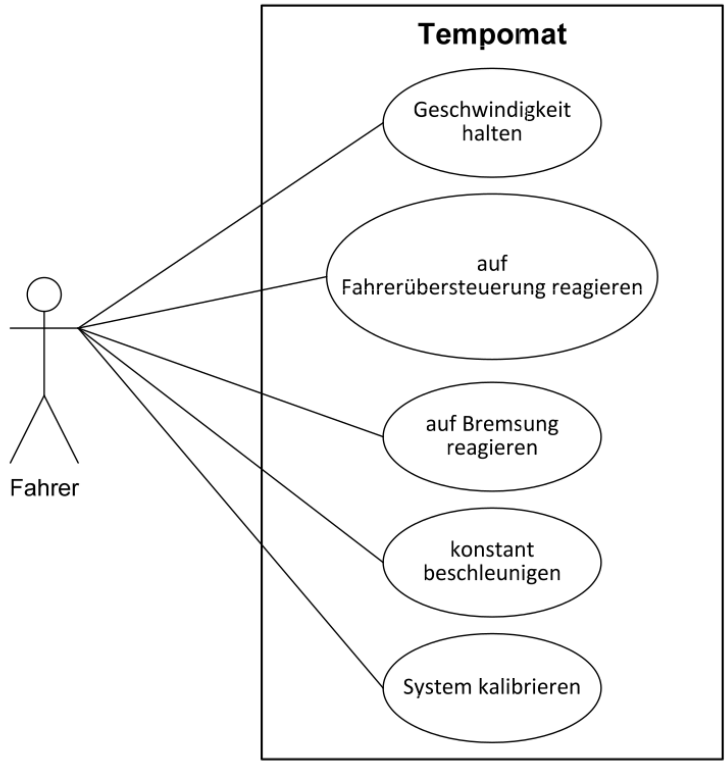
\includegraphics[width=\columnwidth]{images/use-case-diagramm_schlecht.png}
\end{minipage}
\hfill
\begin{minipage}[t]{0.48\columnwidth}
    \myul{\textbf{Tempomat: verbesserte Version}}

    \vspace{0.1cm}

    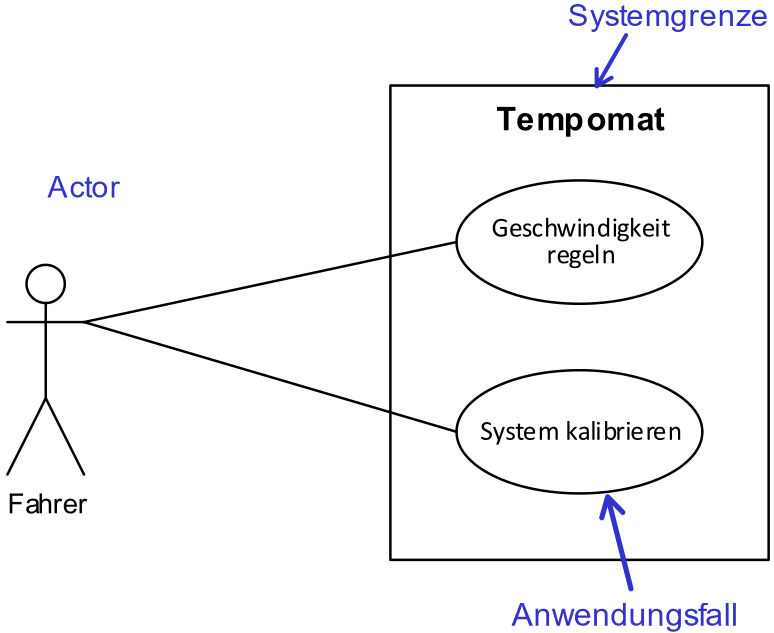
\includegraphics[width=\columnwidth]{images/use-case-diagramm_besser.png}
\end{minipage}


\subsubsection{Kontextdiagramm: Sequenzdiagramm}

\begin{itemize}
    \item Speziell bei Syetemen, deren Grenzen durch \textbf{Nachrichtenflüsse} charakterisiert werden können
    \item Details zu Sequenzdiagrammen siehe Abschnitt % TODO
\end{itemize}


\subsection{Verteilungen festlegen}

\begin{itemize}
    \item Bei Embedded Systems werden häufg \textbf{mehrere Rechnersysteme} verwendet, um die verschiedenen Aufgaben zu erledigen
    \item Rechner sind örtlich verteilt und mittels Kommunikationskanal verbunden \\
        \textbf{\textrightarrow\ Verteilte Systeme (distributed systems)}
\end{itemize}

\vspace{0.2cm}

\begin{minipage}[t]{0.5\columnwidth}
    \raggedright

    \subsubsection{Verteilungsdiagramm}
    
    \begin{description}
        \item[Knoten:] Darstellung der örtlichen Verteilung der Systeme \\
            Knoten können auch hierarchisch aufgebaut sein
        \item[Linien:] Physikalische Verbindungen der Knoten (Netzwerke, Kabel, Wireless, etc.)
    \end{description}
\end{minipage}
\hfill
\begin{minipage}[t]{0.46\columnwidth}
    \example{Tempomat}
    
    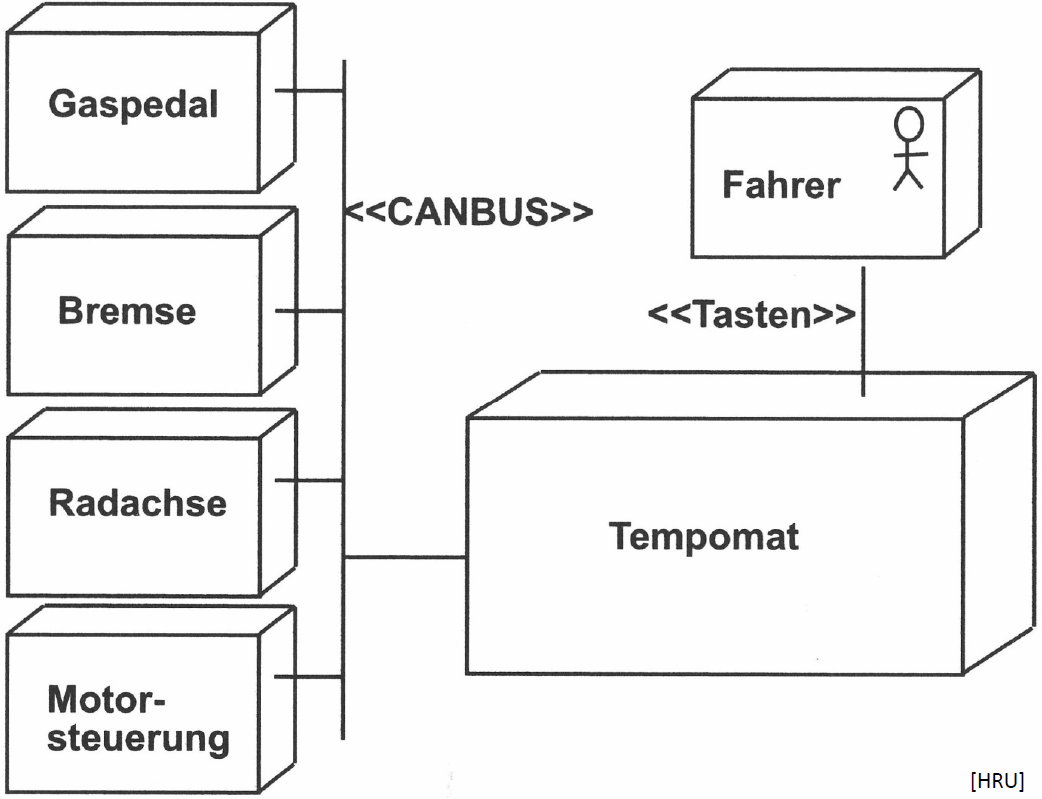
\includegraphics[width=\columnwidth]{images/verteilungsdiagramm_tempomat.png}
\end{minipage}


\subsection{Systemprozesse detaillieren}

\begin{outline}
    \1 Die gefundenen Systemprozesse (use-cases) müssen genauer spezifiziert werden
        \2 \textbf{Nicht detaillierter spezifizieren als sinnvoll / gefordert!}
        \2 Jede weitere Spezifizierung soll eien 'added value' liefern
    \1 Verschiedene Detaillierungsstufen für verschiedene Zielgruppen
        \2 Auftraggeber: Überblick (z.B. in Form von Umgangssprachlichem Text)
        \2 Systementwickler: 'Normale Sicht' enthält mehr Details
\end{outline}


\subsubsection{Sequenzdiagramm}

